\chapter{Extra stuff} \label{ap1:Lorem}
\todo{better name for this chapter}

\section{Exploratory evaluation of ChatGPT's capabilities}

\subsection{Fabricated Examples}

In the initial step of work, we superficially explored ChatGPT's ability to generate tests for an example conflict of Point, where a distance method is altered from euclidean to manhattan in one branch and in the other branch, a move method is changed from using the value 1 for x and y movement to using the result of the distance calculation.

We tested two frameworks, first just asking for a test, with prompts based on the testing indications given by the DSL for the case:

\begin{itemize}
  \item A Dependency Based semantic conflict was possibly introduced in a 3-way merge. Develop a test for the class Point, that covers the methods move() and distance(), without calling distance() directly.
Before the merge, the class under test was: [base Point]
After the merge, it was: [merged Point].
  \item A Dependency Based semantic conflict was possibly introduced in a 3-way merge. Develop a test for the class Point, that covers the methods move() and distance(), without calling distance() directly.
Before the merge, the class under test was: [base Point]
In the branch A it was changed to: [A Point]
In the branch B it was changed to: [B Point]
After the merge, it was: [merged Point].

\end{itemize}

For this, the LLM simply took one version and created tests taking it as correct behaviour. In the first case, for Base and in the second for Merge. This is not ideal, as the first does not allow us to distinguish if the behaviour changed due to merging, or just do to changes in the branches. The latter takes merge as correct behaviour and will thus always fail.

Other tests involved first asking for an explanation if there was a merge conflict there, before asking for a test

\begin{itemize}
  \item We have done a merge on a piece of code.
Before the merge, the code was: [code]

In the branch A it was changed to: [code]

In the branch B it was changed to: [code]

After the merge it was: [code]

Do you believe there could be a merge conflict here? Where? Explain why.
  \item We have done a merge on a piece of code.
  
Before the merge, the code was: [code]

In the branch A it was changed to: [code]

In the branch B it was changed to: [code]

After the merge it was: [code]

Do you believe there could be a merge conflict here? Where? Explain why. Pay attention to both additions and modifications.
  \item We have done a merge on a piece of code code.
  
Before the merge, the code was: [code]

In the branch A it was changed to: [code]

In the branch B it was changed to: [code]

After the merge it was: [code]

Do you believe there could be a *semantic* merge conflict here? Where? Explain why. Pay attention to both additions and modifications.

\end{itemize}

The first two prompts failed. Indeed for prompt ChatGPT only mentioned the changes in move, but even after prompting it to pay attention to distance, it failed to identify the conflict. For both, it seemed to not understand what was being referred to when speaking of conflict, describing all changes as a "conflict". Thus it would say, there is a conflict between whether to use euclidian and manhattan distance and there is a conflict on how the move function works.

The last prompt given, highlighting the *semantic* aspect of the merge conflict, yielded good results, with the conflict being perfectly described, as seen in \Cref{fig:semconf}. After prompting for a test, it generates an appropriate one: it tests if the move function updates Point appropriately based on the euclidean distance. Thus it fails for base and branch B, where movement is still done with the value of 1, it passes for branch A as there move is based on distance; and it fails in merge, as now movement is being done with the distance calculation, but the calculation is now manhattan.

\begin{figure}
    \centering
    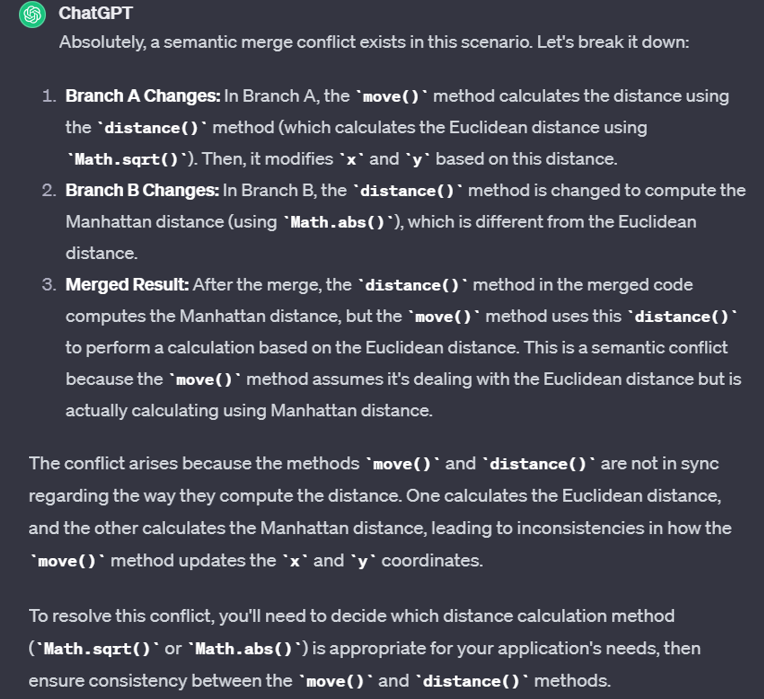
\includegraphics[width=0.75\linewidth]{figures/image.png}
    \caption{ChatGPT description of the semantic conflict.\todo{can we have a white-background of it? or having this in a \texttt{response} environment.}}
    \label{fig:semconf}
\end{figure}

In simple fabricated scenarios, where simple conflicts were added to existing software solutions, ChatGPT showed ability to identify and describe the semantic conflict. Despite this, test generation remained complicated and few of the successful identification of semantic conflicts yielded working tests. The final prompt follows.

\begin{prompt}
Generate a Junit unit test to identify this semantic conflict, knowing what you do now. The test must compile without errors and require no further alterations. It should require no further dependencies and import all classes correctly.
\end{prompt}

While adapted to avoid common pitfalls, the tests generate still suffered from basic issues such as missing imports, which could be mitigated by prompting the LLM for correction automatically. More complex issues of implementation were present, such as calling the base function instead of dependent, wrong usage of construction and function returns, parameter types or unnecessary mocks. Further, when prompting for correction, the LLM often explains that the developer should correct this, thus further work needs to be done to ensure the tool does all the work itself.

\subsection{Real-World Merge Conflicts}

Prompting in real-world examples, or more complex fabricated examples, has produced far worse results. Several refinements were made to the prompts, most significantly: the usage of "git diff" to highlight the specific changes in branch A and branch B, the explanation of the conflict present and the specification of the target method where the conflict is evident. These modifications were largely unsuccessful and did not lead to identification of any significant amount conflicts.

We also had to reckon with size limits for messages. Thus, when necessary, we started with an explanatory prompt and then fed the information step by step. However, it remained crucial to remind the LLM of the goal in the last message.

\begin{prompt}
We have done a merge on a piece of software and introduced a semantic conflict of types: "Update two different dependencies of a method or update one method and concurrently update one of its dependencies" and "Concurrent changes to the same method". I will now show the base commit, the diff in branch A, the diff in branch B, and the final merge version in 4 separate messages. At the end I want you to explain why and where the semantic conflict is present.
\end{prompt}

Common issues are confusion between textual and semantic merges, which can be mitigated by clear explanation of what a semantic merge is; hallucinations of features not present in the code or hallucinations of changes where changes were not made; lack of focus on the methods where conflict is evident, despite reiterations; loss of focus when prompt has to be split into several messages. 
Rare close successes occured, particularly in cases where the conflict was asserted to be there in the prompt and could simply be described by explaining the changes made, such as parallel changes to collections initialization, as seen in \Cref{fig:cantfind}.

\begin{figure}
    \centering
    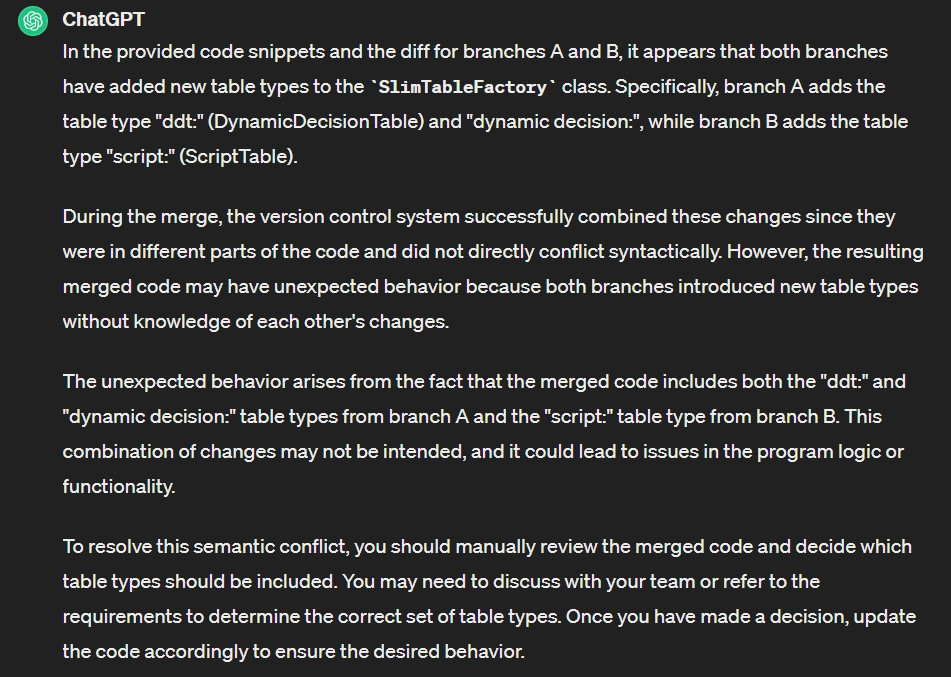
\includegraphics[width=1\linewidth]{figures/almostsemantic.jpg}
    \caption{ChatGPT describes the parallel changes as the origin of the conflict, but falls short of describing the emergent behaviour (in this case as simple as the different value returned by size()).\todo{can we have a white-background of it? or having this in a \texttt{response} environment.}}
    \label{fig:cantfind}
\end{figure}

While we found that ChatGPT could not identify the semantic conflicts present in real software solutions, in some of \citet{kn:nuno}'s fabricated scenarios, these were correctly explained. Part of the difference between real-world examples and fabricated scenarios may come down to the information given. The fabricated scenarios were accompanied with a description of the specific semantic conflict present and the changes made perfectly reflected the description, with clear modifications and no extraneous changes. Thus it is possible collecting and offering that information with real-world scenarios may improve the ability of LLMs in this regard, but the higher "noise" of these scenarios may be too disruptive in this regard.

Another factor in consideration is the issue of dependencies, as so far testing had focused on just a unitary class. Given that semantic conflicts can involve interactions between classes and subclasses or other dependencies, it is relevant to provide further information. Initial tests just added one dependency, whether by calling a class methods or due to a inheritance relationship. An example, with the addition of an illustrative example of a semantic conflict follows.

\begin{prompt}
We have done a merge on a piece of software and introduced a semantic conflict of type Parallel Changes in Method.

Semantic conflicts occur when concurrent and syntactic-correct changes in different regions of a source file or different files cause the software system to misbehave. For example, suppose there is a Java class `Point` with a method `distance()` that computes the Euclidean distance of a Point to the origin and Bob decides to modify `distance()` so it computes instead the Manhattan distance. At the same time, Alice, not aware of Bob's changes, creates a new method `move()` that uses `distance()` to calculate the Euclidean distance. Then, the changes of both developers are merged. As Bob and Alice did not modify the same lines of code, there is no textual conflict. There is neither a syntactic conflict as the merged code still compiles. However, the program now has an unexpected behaviour. The `move()` method introduced by Alice no longer moves a Point an Euclidean distance (as Alice was expecting) but rather moves a Manhattan distance

The affected declaration is copyWithDefaults().

A first message will detail the class before the merge, the diffs for both branches and the class after the merge. A second message will have a dependent class, whose methods indirectly call copyWithDefaults(). After I send these next two classes, identify and describe the semantic conflict.    
\end{prompt}

A more complex evolution on this idea consisted of providing textual representations of UML graphs, such as plantUML call and structure graphs. These however proved to be complex in their own regard as they often induced the LLM to "forget" previous information and its goal, possibly due to their large size. A factor to consider, too, was that the information provided had to be limited in depth since, depending on the size of the software solution, a complete graph would be of extremely unwieldy size. Through some effort, we could get the LLM to recognize both the diagram and the class information, namely, by offering the diagram first.

\begin{prompt}
We have done a merge on a piece of software. In this, we introduced a semantic conflict on the method dominates(State| State) of the class OpenTripPlanner. In a first message I will send a call diagram, in plantUML format. In a second message I will send the original class, the differences in the branches and the merged class.  At the end you must identify and explain the semantic conflict.
\end{prompt}

However, it was particularly necessary to frequently refocus and concentrate the LLM. For example, after sending the diff and class information, reminding:

\begin{prompt}
Explain why and where the semantic conflict is present, taking into account all the information provided in the last 2 messages. As mentioned before, focus on dominates(State| State). Make sure to mention information from the call diagram, if it is relevant to understanding the conflict.
\end{prompt}

In the end, we were able to get the LLM to both recognize the merge information and the call diagram focused on the affected declaration and obtain a correct description of both the meaning of the diagram and the changes made in the merge. This however did not entail any improved description of the conflict, for all the cases tested.

Underscoring these experiments with real world test cases is an overlying issue: to properly identify a semantic conflict, we may have to analyze and take into account a large amount of data across several components of the software, while at the same time focusing on the specific components that were changed. While this is natural to a human, there is no clear way to select which information to feed and which to not in the LLM prompt: while a wider breadth of information may be necessary to identify the conflict, it is extremely likely to just induce further confusion and lead ChatGPT to focus on the wrong thing, or confuse different parts of code or even lose track of the task at hand as mentioned before.

\subsection{Test Generation without Conflict Understanding}

Given the difficulty of getting ChatGPT to provide accurate descriptions of the semantic conflicts, it was worth exploring whether the conflicts can be made evident just by generating tests targeting affected methods and classes. Several strategies were adopted: the prompting with the class after merge, the prompting with the class after merge and branch diffs and prompting with the class after merge and a structure graph. In most cases, where existing test suites where available, such information was also provided, with the prompt being reformulated to ask for its extension, rather than generation from scratch, as this shown to be important before~\cite{kn:githubcopilot}.

For 15 tests of 5 different projects, only 2 compiled, before and after prompting for corrections. One of these tested trivial additions to an array in both branches and the other identified a behaviour introduced in branch B that successfully carried over to merge, thus not a conflict. Positively, ChatGPT could understand the significance of this test working in branch B and merge but not A, as seen in \Cref{fig:testexplain}, suggesting it could understand the significance of a test failing for merge but not upper branches, which would indicate conflicts.

\begin{figure}
    \centering
    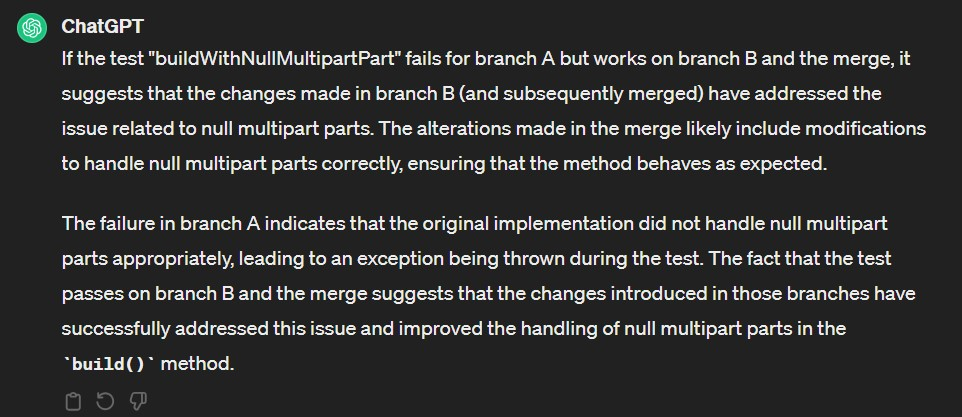
\includegraphics[width=1\linewidth]{figures/testexplain.jpg}
    \caption{ChatGPT explanation of meaning of failures and passes of test in different branches.\todo{can we have a white-background of it? or having this in a \texttt{response} environment.}}
    \label{fig:testexplain}
\end{figure}

Common issues affecting test generation were:

\begin{itemize}
  \item Faulty importing/setup: Particularly relevant in the OKHttp case, the tool was patently unable to correctly call imports, just omitting them, even when expressly being given the package names and being told to import it.
  \item Invalid access: The LLM was generally unable to distinguish between private and public methods and frequently made attempts to invoke or access private methods and fields.
  \item Method/Field/Class Hallucination: ChatGPT frequently invoked non-existent methods, fields or even classes. In some classes this could also be related to matters of access, as it generated getter calls for private fields.
  \item Incomplete/Template Tests: Despite being prompted explicitly to generate complete tests that should compile, in several cases tests were generated with incomplete template helper methods and classes.
\end{itemize}

While feeding compilation error outputs could be a solution for these, in practice no test that failed to compile was fixed in this manner, as changes made did not fix or ignored the problems present. In some cases, while the logic of correction was sound logically, they were not helpful in the context of automatic test generation. For example, a "MockConverter" class was used in a test for the Retrofit project. Upon prompting for a fix, an import was added, which still naturally was non-functional. Upon prompting for another fix, ChatGPT provided a basic empty template for the MockConverter class. While a correctly implemented MockConverter class would fix the issue and allow the test to compile, the solution here would have been to drop the usage of the MockConverter class in the first place

Experiments were made to employ the usage of vector indexing to boost the capabilities of understanding code. The theory was that, by indexing the entire repository of code, we could proceed with prompting without having to decide which specific blocks of code should be required information in the prompt and that, during generation, the LLM could correctly identify the chain of dependencies, and which methods and parameters should be employed to properly test our desired methods. In this process we employed llama\_index, but the results fell short: due to an observed worse ability to generating code, focus was placed on the explanation of what should be done, with the prompting: "We want to create an extensive testing suite for the method [method] of the class [class]. How should we approach this? Which calls should we make, which parameters should we try and which results should be expected?"
Results were generic, many times not even referring to aspects of the code itself and still prone issues of hallucination, specifically the making of references to non-existent methods.

\section{Comparison of Developed Prompts with State of the Art}

To evaluated our progressively developed prompt with existing state of the art, we selected 5 prompts from comparison, henceforth referred as 1 \cite{kn:chattester}, 2 \cite{kn:siddiq2023empirical}, 3 \cite{kn:gptunitbra}, and 4 \cite{kn:chatunitest}. Our prompt, in turn, was 2-step prompt as follows:

\begin{prompt}
The following class was altered in a merge, specifically the METHOD method. Analyse it and what it does, with focus on the method and its usage: CLASS INFO
\end{prompt}

\begin{prompt}
You are a Java developer. Due to changes in the METHOD method, you've been asked to write a complete test suite to identify possible errors introduced due to the changes. Write a junit test suite for the method. All classes must be correctly imported. The tests must compile without errors. The tests must be complete and require no modification and addition. No explanation needed.
\end{prompt}

As subjects, we selected the basic fabricated Point class example, Antlr4, whose testing simply requires the length of a returned list and OkHttp, a more complex example requiring mocks and reflection for testing.
For each prompt, we generated 3 times and selected the best result for comparison.

For Point, we made the following observations:

Our prompt generated a suite with 3 tests, one of which had an incorrect assertion (A Point with coordinates -3,-4 was expected to move to 4,5 when it should move to 4,3). Despite this one wrong test, the correct ones successfully identified the conflict, as they tested manhattan distance movement. For an earlier branch, with euclidian distance movement, they would fail, showing the conflict.

Prompt 1 called the distance() method to identify where the Point should be and set assertions accordingly. While this tested the move method, it could not identify the conflict, as the assertions were dependent on the behaviour of distance(), as it changed so did they.

Prompt's 2,3,4 all made the same mistake: Starting from a point 3,4, they expected it to move to 7,8. As distance is 7, it should actually move to 10,11. Notably, Prompt 3 and 4 generated tests for distance and correctly identified it as 7.

For Antlr4, our prompt ran into errors: it could not correctly initialize the class, as the CodeGenerator object called by the constructor was incorrectly created. It also severely undercounted the number of keywords, leading to an incorrect assertion.
Prompt 1 showed improvement over ours, as it understood a null could be used in place of CodeGenerator, as it would not be used for our purposes. Despite this, it failed in the logic of the test, calling badWords unnecessarily: this is a private method that is already called by the getBadWords method we are testing. This same error was present in Prompt 2.
Prompt 3 generated nonsensical tests, just checking if the result of methods called was false. While it tested non-existent methods, it did not tested getBadWords as we desired.
Prompt 4 also called addBadWords despite not needing it, but as it was instructed to use Mockito, it avoided the error of calling a private method by using reflection. The rest of the test logic and the assertion was correct.


OkHttp should be the hardest to test, as the method under test and the method which calls it are private. The value returned (which we seek to test) is never publicly available.
Thus all prompts try and fail to call the private method. The exception is Prompt 3 which, by it's nature of generating for all methods rather than being told to generate for a specific one, avoids private methods. Surprisingly, Prompt 4 which had shown ability to use reflection in the previous subject, failed to produce a satisfactory result. Also of note is Prompt 2, which calls for 10 tests to be generated: in this case, to reach this 'quota', each parameter of the copied client was tested in a entirely different test, rather than just in a different assertion.
Despite failing, due to previously mentioned issue with access, Prompt 1 notably produced the best assertions, as it tested both functionalities of the method: the correct copying of defined parameters, and the returning of defaults for parameters that were not set.
